\subsection{Datasets}
\label{sec:datasets}


\begin{figure*}
\begin{center}
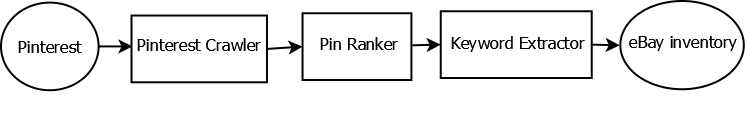
\includegraphics[height=2.5cm]{figures/Pipeline.png}
\caption{Pipeline for generating interesting eBay products based on Pinterest. Pinterest is first crawled, next the pins will be ranked and filtered based on whether or not they contain useful product information, next a product keyword extractor is applied to a set of highly ranked pins, and finally the extracted keywords are used to find a relevant eBay product.}
\end{center}
\label{fig:pinterest-pipeline}
\end{figure*}

We used the following two datasets in our experiments: 

{\bf Interesting iPhone cases}.
In this dataset, we generated a collection of interesting (positive) and uninteresting (negative) iPhone cases as follows. For positive generating positive examples, one natural choice was exploiting the data hosted by Pinterest. By definition, it is fair to assume that anyone who pins a product on Pinterest has found it interesting to some degree. The more a pin is engaged by the users, the more interesting is the product to those users. Although Pinterest data is biased by the demographic of its users, it is a publicly available dataset and is a more natural choice compared to collecting interesting products using crowd sourcing such as  {\em Amazon Mechanical Turk (AMT)} where it would be more subject to demographic biases. We built a pipeline for generating interesting eBay products illustrated in Figure~\ref{fig:pinterest-pipeline}.  In the first stage, we periodically crawl pins from Pinterest. In the next stage we filter the pins which do not have rich textual content and then rank the remaining pins using a score computed from the number of {\em repins}, {\em likes}, and {\em comments}. In the next stage, we trained a {\em Conditional Random Field (CRF)} model for extracting product related keywords from a set of highly ranked pins produced in the previous step. The final set of product related keywords  is then used to find a match in the eBay inventory. 

For generating the uninteresting iPhone case dataset (negative examples), we
hired workers from {\em AMT} to label a collection
of nearly 20,000 iPhone cases on {\em eBay}.  We then pulled our final dataset from the annotated by selecting only those instances where the annotators all labeled it as uninteresting. 

The final data-set consists of $2179$ positive and $9770$ negative instances
for a total of $11,949$ instances. For each instance, the product title of
the corresponding {\em eBay} listing was used as the input. In this case we are
dealing with very short text snippets, usually 10 to 12 words each. To
train a topic model, we used a larger, more broader set of about
$2$ million product titles, grouped based on {\em eBay} categorical information into about $8,000$
documents of approximately $200$ titles each.


%{
We used insights from 
interesting iPhone cases found on {\em Pinterest} and {\em eBay's}
user behavior data in order to generate a balanced data-set.  
We then pulled our final dataset from the annotated by selecting only
those instances where the annotators all labeled it as 
positive (i.e., interesting) or negative (i.e., uninteresting). The
final data-set consists of 2179 positive and 9770 negative instances
for a total of 11,949 instances. For each instance, the product title of
the corresponding {\em eBay} listing was used as the input. In this case we are
dealing with very short text snippets, usually 10 to 12 words each. To
train a topic model, we used a larger, more broader set of about
2 million product titles, grouped based on {\em eBay} categorical information into about 8,000
documents of approximately 200 titles each.
%}

{\bf {\em NSF} abstracts}. For the second dataset we used a set of
61,902 National Science Foundation 
Scholarship proposal abstracts (see~\cite{bache:2013} for more
details) to evaluate how our diversity measure 
compares to other methods on larger pieces of text. We used this set
for training a topic model, however to get labeled data, we had to
generate artificial examples, by randomly mixing pairs of abstracts that we
could expect to be either similar (small diversity) or very different
(high diversity), based on the available meta-data, and labeling them accordingly. We generated 5,000 of
those examples with positive and negative labels evenly represented. For both datasets, we used the Mallet LDA implementation and learned a separate topic model with $400$ topics.

\begin{table*}[t]
\label{tab:classification-results}
\vspace{4mm}
\begin{center}
\begin{tabular}{|l|c|c|c|c|}
\hline
&Precision & Recall & F1 & Accuracy
\\ \hline 
JSD Features         &$\mathbf{0.714}\pm 0.015$&$0.597\pm 0.016$&$0.650\pm
0.014$& $\mathbf{0.8828}\pm 0.0045$\\
RAE             &$0.676\pm 0.005$&$\mathbf{0.666}\pm 0.030$&$\mathbf{0.671}\pm
0.013$&$0.8809\pm 0.0020$ \\
SVD Features             &$0.676\pm 0.008$&$0.633\pm 0.017$&$0.654\pm
0.010$&$0.8778\pm 0.0027$\\
\hline
\end{tabular}
\caption{Classification results for the eBay dataset.}
\end{center}
\end{table*}

\subsection{Unsupervised Learning}
\label{sec:unsupervised-learning}

We evaluated our text diversity model in an unsupervised learning task
on both datasets.
We implemented our model by combining the topic similarities with the
Reader's model (labeled by {\em JSD-Sim-Con}) and compared it against a few
baselines: Shannon entropy, Rao Diversity and a measure
based on Determinantal Point Processes.
The Shannon entropy has
been previously tested as a measure of document diversity with quite
underwhelming results in \cite{bache:2013}, where the authors proposed 
Rao diversity as a better solution, which incorporates the topic similarity
information to provide better accuracy. We asked the question whether
the poor performance of entropy might be due to a suboptimal choice of
topic distribution, which led to our topic similarity
method. This technique can be used on any topic distribution
by simply multiplying it by the topic similarity matrix, and then
renormalizing. We present the performance of entropy with - and
without - the topic
similarity transformation to verify that this approach improves the results not
only for Jensen-Shannon Divergence, but for other measures as well.
Both for the entropy and Rao diversity, we generated topic
distributions by inferring them for each instance, based on the LDA
model, using the standard functionality from Mallet.

Determinantal Point Processes (DPP) have recently gained popularity as a
useful tool for sampling diverse subsets, with many applications
(see~\cite{kulesza:2012} for more details). We were interested to see
if they can also be useful for 
measuring the diversity of a set provided as input. Given a set of
instances described as feature vectors $U=\{v_i\}_{i=1}^N\subset \rr^T$, DPP defines a
sampling model for selecting a subset of $S=\{v_{i_j}\}_{j=1}^k$, by
setting the probability of $S$ proportional to the determinant of the
Gram matrix corresponding to those vectors. One might therefore
consider this determinant to be a good measure of set diversity,
because, intuitively, a more diverse set should have a higher
probability. The problem with this, however, is that determinants are
computationally unstable and very sensitive to local changes. For
example, if any two instances happen to have identical vector
representations, that immediately forces the determinant to $0$, even
though a set may be otherwise very diverse. We decided to use
another measure derived from a DPP. Instead of looking at a set $S$
(in our case, a set of words) as a sample from a larger set, we can
imagine sampling from $S$ itself. In that case, the average size of
the samples tells us how many significantly different words there are
in the given text. Fortunately, the expected sample size can be
computed from the eigenvalues of the aforementioned Gram matrix, as
discussed in \cite{kulesza:2012}. Two aspects of the feature
vectors are relevant for the DPP. The length of the vector represents
the relevance of the corresponding word, while the direction is
responsible for determining the pairwise similarities. For the
direction, we used the distributional representations from the
Reader's model. For the vector lengths, we tried two versions: all
unit lengths (i.e. no preference), and using the importance values from
Definition \ref{mixture}. One drawback of the expected
DPP sample size is that it is correlated with the length of a
document. However, within each of our datasets, the instances have roughly
similar length.

Figures \ref{fig:roc-curves} (a) and (c)
present ROC curves comparing all of the diversity measures for each dataset.
In either case it can be observed
that our approach outperforms the other baselines, with an AUC
around $0.73$. Moreover, for the {\em eBay} dataset the other measures
give poor results. This can be explained as follows: since the
text snippets are short, the LDA may yield a poor topic inference for
such short text and as a result all measures using topic inference
would perform poorly. The DPP-based measure does have some correlation
with the labels for both datasets, although not particularly
high. Interestingly, for the eBay dataset, unit vector lengths
performed better, while for NSF, importances gave an improvemet (in
each case, only the better result was
plotted). Another interesting observation is that comparing the
results for entropy with - and without - topic similarity for the NSF
dataset, shows that this technique provides as much - if not more -
improvement as does Rao diversity over regular entropy.
\begin{figure}
\begin{center}
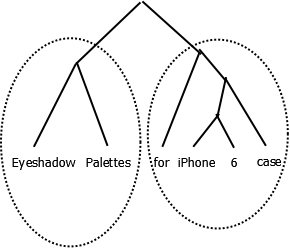
\includegraphics[width=5.5cm]{figures/RAE.png}
\caption{RAE tree learned for the product: {it Black Qi Standard Wireless Charging Charger Receiver Case For iPhone 5 5G}. Note how RAE learns to merge different concepts separately and merges them until very last step into the root node.}
\end{center}
\label{fig:rae-example}
\end{figure}

Figures~\ref{fig:roc-curves} (b) and (d)  
show the gains we obtain by applying topic
similarity and context conditioning techniques that we
discussed in Sections~\ref{sec:the-readers-model} and
\ref{sec:topic-similarities}. Both methods appear to be beneficial,
significantly improving the AUC. Interestingly, using
topic similarities appears to skew the ROC curve towards the upper
right, while context conditioning gives more improvement in the lower
left corner of the plot. We also measured the difference between using 
the Informative Mixture and simply taking a uniform mixture of
distributional representations. The importances appear to have a
particularly significant effect for the NSF dataset - probably because
the larger size of documents makes it necessary to effectively ignore all of
the irrelevant words.

\subsection{Text Embeddings}
\label{sec:text-embeddings}

In the second set of results, we used an unnormalized version of the Informative Mixture
distribution (described in Definition~\ref{mixture}) computed over
{\em eBay} product titles in a supervised classification
setting for both datasets described in Section~\ref{sec:datasets}. We also used two 
different baselines for comparison. For the first baseline we used {\em Latent Semantic Indexing (LSI)} features by forming a
document-term matrix and performing SVD. For the second baseline we used the {\em recursive auto-encoders (RAE)}~\cite{Socher:2011:SRA:2145432.2145450}. RAEs 
have been shown sucessful for sentence-level prediction of sentiment label
distributions. There is a nice connection between RAEs and text diversity: starting from the word level, an RAE greedily forms substructures that yield the least reconstruction error  structured in a  binary tree. As a result at the higher levels of the tree we observe the more diverse  substructures. This is further illustrated in Figure~\ref{fig:rae-example} where it shows the learned RAE structure for the example product shown in Table~\ref{tab:ebay-interesting-products}(a). When RAE is applied to the product title "Eyeshadow Palettes for iPhone 6 case" , we can observe that the words \{for, iPhone, 6, case\} are combined into one substructure, while the words \{Eyeshadow, Palettes\} form a different substructure. In other words RAEs inherently respect diversity at higher levels of the RAE tree structure.

Table~\ref{tab:classification-results} shows
the performance of the SVM classifier using our proposed mixture topic
distribution as features and compares it to these different baselines.
These results are averaged over five different cross-validation splits using $0.6$ for training
and $0.4$ for testing. Our proposed approach shows a higher precision
and a marginally higher accuracy compared to the baselines.
